\documentclass{article}
\usepackage[a4paper, margin=1in]{geometry}
\usepackage{setspace}
% \usepackage{parskip}
\usepackage[backend=biber, sorting=none]{biblatex}
\usepackage{graphicx}
\usepackage{float}
\usepackage{tocloft}
\usepackage{chemfig}
\usepackage{nameref}
\usepackage{hyperref}
\usepackage{tabularx}
\usepackage{multirow}
\usepackage{hhline}
\usepackage{booktabs}
\usepackage{subcaption}
\usepackage{amsmath}
\usepackage{amssymb}
\usepackage{amsfonts}
\usepackage{amsthm}
\usepackage[group-separator={,}]{siunitx}

\addbibresource{main.bib}
\graphicspath{ {./images/} }

\renewcommand{\arraystretch}{1.2}

\DeclareMathOperator*{\argmax}{argmax}
\DeclareMathOperator*{\argmin}{argmin}
\DeclareMathOperator*{\softmax}{softmax}

\newlistof{equations}{equ}{\normalfont\Large\bfseries List of Equations}
\newcommand{\equationname}[1]{%
    \begingroup
        \leavevmode
        \addcontentsline{equ}{equations}{\protect\numberline{\theequation}#1}%
    \endgroup   
}
\setlength{\cftequationsnumwidth}{2.5em}
\setlength{\cftequationsindent}{1.5em}

\begin{document}
\doublespacing

% \begin{figure}
%     \begin{subfigure}{0.49\textwidth}
%         \centering
%         \includegraphics[width=\linewidth]{}
%         \caption{}
%     \end{subfigure}
%     \caption{}
% \end{figure}

% \textbf{Discussion points for this section:}
% \begin{itemize}
%     \item 
% \end{itemize}

\begin{titlepage}
    \centering
    \singlespacing
    \vspace*{1cm}

    
\includegraphics[width=0.2\textwidth]{University_of_Canterbury_logo.svg.png}\\[1.5cm]

    \Huge
    \textbf{COSC681 - AI Project}\\[1.5cm]

    \LARGE
    Classifying smoking exposure with epigenetic-trained machine learning\\[2cm]

    \Large
    \textbf{Lachlan Jones}\\[0.5cm]
    2025\\[1cm]

    \large
    \textbf{Supervisors:}\\
    Prof. Greg Jones (University of Otago)\\
    Prof. Richard Green (University of Canterbury)

    \vfill

    \Large
    Department of Computer Science\\
    University of Canterbury
\end{titlepage}

\pagenumbering{roman}

\begin{abstract}

\end{abstract}

\newpage
\tableofcontents

\listoffigures
\listofequations
\listoftables

\newpage
\pagenumbering{arabic}

\section{Introduction}
\subsection{Tobacco-related health issues}
The harms associated with tobacco use are well recognised. Tobacco kills up to half its users who do not quit and more than 8 million people per year, including an estimated 1.3 million non-smokers due to second hand smoke \cite{who_tobacco}. Smoking causes cancer, heart and lung disease, stroke, type 2 diabetes, and harmful reproductive effects \cite{hhs_smoking_2014}. There is a growing body of evidence suggesting a causal relationship between smoking and mental health issues \cite{taylor2019smoking}. Clearly, such negative impacts on patient health due to tobacco use are undesirable, just as they are avoidable. For these reason, tobacco usage is of great concern to health professionals. The World Health Organization asserts that surveillance is key for addressing the tobacco epidemic, as tracking tobacco usage indicates how to shape policy \cite{who_tobacco}.

\subsection{Self-reported smoking status}
Current- surveillance relies on self-reported smoking data. That is, a patient's smoking history is recorded by them personally recalling and reporting. It is a convenient and cost-effective way of collecting smoking statistics. There are two main types of smoking data used to measure tobacco exposure: smoking status and smoking pack-years. Smoking status is label based on the history and habits of tobacco use. Individuals are binned into never-smokers, ex-smokers and current-smokers. Smoking pack-years is a calculated score that tries to quantify tobacco use. It is calculated as the number of packs of cigarettes smoked per day multiplied by years of smoking \cite{smokingpackyears}. For example, one pack-year is one pack per day for one year, or half a pack per day for two years. Therefore, smoking pack-years quantifies both the degree of exposure and duration of exposure equally.

Self-reported smoking data has several limitations. Relying on individuals recounting information can introduce bias. Self-reported smoking data is prone to inaccuracy due to stigma, recall bias and a lack of information on second-hand exposure \cite{park2015correlation, gorber2009accuracy}. That is, the social pressure to deny partaking in stigmatised behaviours, forgetting details and information, and not being aware of sources of second-hand exposure can all influence the results of self-reported smoking data. A method of using objective evidence to determine smoking history could overcome these issues. On the other hand, the inaccuracy of self-reported smoking data can differ between population groups. For example, studies suggest that teens are more likely to provide false responses in smoking surveys \cite{park2015correlation}. Moreover, tobacco consumption differs between social groups, with smoking more prevalent in low-education and low-socio-economic groups \cite{cdc2019_smoking}.

To this end, developing diagnostic tests to collect smoking data that do not share the biases of self-reported methods are of interest for improving the monitoring of health. One such approach is the use of epigenetic biomarkers.

\subsection{Epigenetics}
Epi- is a Greek prefix meaning upon or on. Therefore, epigenetics is the study of factors on top of or upon genetics. Specifically, it is the study of how environmental factors and behaviours affect, modify and regulate your genetics and their expression, without changing the DNA itself. We consider one type of epigenetic modification: DNA methylation.

\begin{figure}
    \centering
    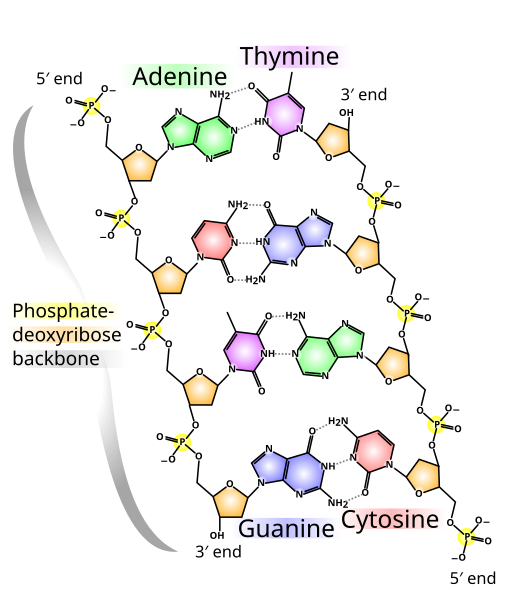
\includegraphics[width=0.5\textwidth]{512px-DNA_chemical_structure.svg.png}
    \caption*{Chemical structure of DNA \cite{ball_DNA_structure}}
\end{figure}

\subsubsection{DNA methylation}
DNA is a sequence of one of four nucleotide bases: adenine (A), cytosine (C), guanine (G) and thymine (T), linked together by a deoxyribose sugar and phosphate backbone. It is this sequence that provides genetic instructions. Like a human reading a book, strings of these bases are converted into information that tells cells how to function, called DNA transcription. Continuing the book analogy, a sentence of such instructions is called a gene, found in a chapter called a chromosome.

DNA methylation involves the addition of a methyl group (CH\(_3\)) to the 5-carbon position of cytosine nucleotides. This cytosine modification makes it harder for transcription to occur, which can modulate, or even completely silence, gene expression. This is relevant when a guanine is directly followed by a cytosine in the DNA sequence. Because of the phosphate connecting these bases, such a region is called a CpG site. CpG sites are the main form of DNA methylation that occurs in mammalian cells.

A biological sample used to assess DNA methylation will contain many thousands of copies of DNA. When measuring a CpG site for DNA methylation, the reported value is the percentage of DNA copies from the sample which are methylated. That is, a value between 0 (all DNA copies unmethylated) and 1 (all DNA copies methylated).

% At a high level, DNA is a sequence of letters that provide genetic instructions. Like a human reading a book, strings of these letters are converted into information that tells cells how to function. More precisely, these letters are one of four nucleotide bases: adenine (A), cytosine (C), guanine (G) and thymine (T). To form the sequence, these bases are attached to a deoxyribose sugar and connected by a phosphate molecule, called the sugar-phosphate backbone. Of relevance is the phosphate molecule, specifically for when a cytosine is directly followed by a guanine in the sequence. A phosphate bonding a cytosine and a guanine (called a CpG site) creates a chemical structure which allows methyl groups to attach. This process is an epigenetic modification called DNA methylation (DNAm). As a biomarker, we measure methylation at a CpG site as a float between 0 and 1, measuring the percentage of methylation at that site.

While the genetic sequence of DNA is stable, methylation is not. It is a dynamic state that depends on factors such as behaviours and environmental exposure \cite{greenberg2019diverse}. Exposure to a wide range of environmental factors including air pollutants \cite{martin2018environmental}, diet \cite{ma2020whole}, physical activity and even psychosocial stress \cite{opsasnick2024epigenome} have been shown to be associated with specific changes in DNA methylation. Additionally, sufficient lack of exposure to such factors can reverse such changes. As previously mentioned, DNA methylation affects the expression of genes. Methylation at a CpG site can silence the expression of the gene that site is located in, where more methylation at a site leads to stronger silencing. Moreover, DNA methylation is not random. There is strong correlation between methylation of specific sites with specific factors \cite{ewasatlas}. In the context of this work, smoking is strongly associated the methylation of cg05575921, found in the aryl hydrocarbon receptor
repressor (AHRR) gene \cite{reynolds2015dna}. With these points in mind, this means that DNA methylation of CpG sites can be used as a biomarker indicative of the factors that caused it, while also describing changes in cellular function. Therefore, DNA methylation is a biomarker not only useful for reporting on environmental exposures, but also predicting future health outcomes or risks. Examples of this include prediction of cardiovascular diseases \cite{cameron2023dna}, neurological diseases \cite{cells11213439}, type 2 diabetes \cite{cheng2023development}, pace of ageing \cite{10.7554/eLife.73420}, and cancer \cite{luo2020circulating}. Furthermore, DNA methylation is not self-reported, and therefore overcomes the biases associated with self-reported data.

Altogether, this motivates the use of DNA methylation data to develop methods for collecting smoking history of individuals. Work using such data is referred to as an epigenome-wide association study (EWAS).

\begin{figure}
    \setcounter{figure}{\numexpr\value{figure}-1}
    \begin{subfigure}{0.49\textwidth}
        \centering
        \hspace*{11mm}
        \chemfig{*6(-\chembelow{N}{H}-(=O)-N=(-NH_2)-=)}
        \vspace{3mm}
        \caption{Cytosine}
    \end{subfigure}
    \begin{subfigure}{0.49\textwidth}
        \centering
        \chemfig{*6(-\chembelow{N}{H}-(=O)-N=(-NH_2)-(-H_3C)=)}
        \vspace{3mm}
        \caption{5-Methylcytosine}
    \end{subfigure}
    \caption*{Modification of Cytosine into 5-Methylcytosine caused by DNA methylation}
\end{figure}

\subsubsection{DNAm platforms}
The human genome contains \(\sim\!28\) million CpG sites. This is often a computationally infeasible domain for a dataset, due to massive dataset sizes, processing requirements, and noise contained in the signal. Instead, most EWAS use a biologically relevant and informative subset of CpG sites. There are two commonly chosen platforms used to achieve this: Illumina 450k \cite{illumina2012methylation450} and Illumina EPIC \cite{illumina2015methylationepic}. 450k was the first array developed by Illumina, consisting of \num{485577} CpG sites chosen for their quality and usefulness. The EPIC array was developed as a successor, increasing to \num{865859} CpG sites. However, only around \(>90\%\) of the sites were retained from 450k. This is something that needs to be considered when developing scores or screening tests from an EWAS if compatibility with multiple datasets or cohorts is of concern (see \ref{sec:pre-processing}).

Additionally, these arrays are compatible with DNA from multiple different cell types. Some examples include whole blood, purified cells and fresh-frozen tissue \cite{bhat2022data}. Moreover, the methylation signal can differ across different cell types \cite{huang2016epigenome}, which means selection of cell type can be an import factor when designing an EWAS. Typically, whole blood is used, specifically white blood cells, as red blood cells in humans do not carry a copy of the DNA.

% \vspace{1cm}
% \begin{itemize}
%     \item At a high level, DNA is a sequence of letters that provide genetic instructions
%     \item nucleotide bases (A, T, C, G) connected with a phosphate sugar backbone
%     \item Cs next to Gs create a chemical structure that allows methyl groups to attach: CpG site, = epigenetic modification
%     \item description of what the word epigenetics, "upon" genetics
%     \item While genetic sequence is stable, methylation is a dynamic state which depends on factors, enviroment etc.
%     \item The state of methylation can change/effect the expression of genes, where methylation = silencing.
%     \item Methylation isn't random, with strong correlation between methylation of specific CpG sites with specific factors
%     \item This means methylation status can be used as a biomarker for indicating and reporting on environmental exposures and report on health outcomes
%     \item Status of methylation sites can determine health outcomes, including cancer risk, CVD, diabetes, etc.
% \end{itemize}

% \subsubsection{DNAm Platforms}

% \begin{itemize}
%     \item Two types of DNAm platform, illumina 450k and illumina EPIC
%     \item \(\sim\)28 million CpG sites in the human genome, platforms choose specific sites to ranked
%     \item Cell type of sample matters, different cells with have different methylation. Typically whole blood is used, good general methylation signal.
% \end{itemize}

\subsection{Machine learning in epigenetics}
Broadly, machine learning algorithms are split into one of two tasks: regression or classification. The most significant distinction between these two tasks is the choice of supervised learning labels. Regression algorithms are trained against continuous, numeric scores, while classification algorithms are trained against discrete class labels. The choice of label in turn determines the output produced by the algorithm.
Machine learning has already seen use in many areas of clinical epigenetics. We begin with a review of some developed methods, addressing both classification and regression tasks.

\subsubsection{Applications} \label{sec:ml-examples}
\begin{enumerate}
    \item Malta et al. \cite{malta2018machine} proposed a method for assessing oncogenic dedifferentiation (cells becoming cancerous). This approach seeks to model a "stemness index" which indicates how similar a cell is to stem cell - a trait found in cancerous cells. Of relevance is the developed epigenetic approach using one-class logistic regression. The training features consisted of 219 hyper-methylated CpG sites associated with stem cells. Training data only consisted of a single, positive, class: stem cells. The resulting model can then be fed non-stem cells to compare how similar they are to stem cells, i.e. cancerous cells.

    \item Adorj\'an et al. \cite{adorjan2002tumour} proposed a method for using DNA methylation to classify cancer tissues. CpG sites were ranked using a two sample t-test, and then fed into a support vector machine. Models were evaluated using the average of 50 runs of 8-fold cross-validation. The top two CpG sites could classify leukaemia from healthy cells with 84\% accuracy, while the top 60 sites achieve 94\% accuracy.

    \item Dogan et al. \cite{dogan2018integrated} proposed a method for integrated genetic and epigenetic classification of coronary heart disease. The training dataset consisted of 1,545 individuals. An approach combining undersampling and ensemble learning \cite{liu2008exploratory} was used to address class imbalance, creating 8 training sub-datasets. Point biserial correlation and Pearson correlation were used for feature selection, resulting in 107,799 CpG sites for training. These features were ranked using ROC AUC. Random Forest classifiers were then trained on the 8 training sub-datasets, with majority voting used for ensembling. Hyperparameters were tuned using 10-fold cross-validation. The final model used 4 CpG sites, two genetic variables, age and sex. This achieved an accuracy, sensitivity and specificity of 78\%, 0.75 and 0.80, respectively.

    \item
\end{enumerate}

\subsection{Smoking algorithms}
In the context of smoking, the two most significant machine learning epigenetic scores use Elastic Net regression.

\subsubsection{Elastic Net regression}
Elastic Net \cite{zou2005regularization} is a regularised form of linear regression that includes two additional penalty terms.
Given \(n\) examples, \(p\) features with data \(x \in \mathbb{R}^{n \times (p + 1)}\) and corresponding ground-truth \(y \in \mathbb{R}^n\), we find coefficients \(\beta \in \mathbb{R}^{p + 1}\) that produces an output:
\[\hat{y} = x \beta \in \mathbb{R}^{p + 1}\]
and minimises the function:
\begin{equation} \equationname{Elastic Net linear regression}
    \mathcal{L}(y, \hat{y}, \beta) = ||y - \hat{y}||_2^2 + \lambda\alpha||\beta||_1 + \lambda\frac{1 - \alpha}{2}||\beta||_2^2
\end{equation}
where
\[||\beta||_1 = \sum_{i=1}^{p} |\beta_i|\]
and:
\[||\beta||_2 = \sqrt{\sum_{i=1}^{p} \beta_i^2}\]

We can see this is simply mean-squared error, with the \(L_1\)-norm and \(L_2\)-norm included as penalisation terms on \(\beta\). The two hyperparameters \(\lambda\) and \(\alpha\) control the strength of regularisation and ratio between \(L_1\)-norm and \(L_2\)-norms, respectively. Elastic Net is a combination of two other modifications to linear regression: lasso \cite{tibshirani1996regression} and ridge \cite{hoerl1970ridge} regression. The two mathematical regularisation terms have interpretable effects on the convergence of \(\beta\). Gradient updates for \(||\beta||_1\) are uniform for all non-zero values of \(\beta_i\), which typically results in most \(\beta_i\) set to zero, with some having large values. This is referred to as a sparse solution. Gradient updates for \(||\beta||_2^2\) are large for large \(\beta_i\), and small for small \(\beta_i\), which typically results in all \(\beta_i\) having similar values. This is referred to as shrinkage. Together, this results in Elastic Net models promoting the grouping effect, where strongly related features are all included or excluded together. This grouping effect is particularly useful when \(p > n\), as it provides better feature selection than lasso \cite{zou2005regularization}. Because of this, Elastic Net sees wide use in epigenetics, with biological age clocks being one area of particular use \cite{teschendorff2025epigenetic}.

\subsubsection{DNAmPACKYRS} \label{sec:dnampackyrs}
Lu et al. \cite{lu2019dna} proposed DNAmPACKYRS as a DNA methylation based score for calculating smoking pack-years. This score was originally developed as surrogate biomarker for use in the DNAm GrimAge and DNAm GrimAge v2 epigenetic clocks \cite{lu2019dna,lu2022dna}. DNAm GrimAge is a regression model for estimating mortality risk. The DNAm GrimAge score is calculated using covariates sex, age, 7 surrogate biomarkers of plasma proteins, and of relevance, the surrogate biomarker for smoking pack-years: DNAmPACKYRS. Elastic Net regression was used to train both DNAm GrimAge and the surrogate biomarkers of plasma proteins and pack-years. Training data consisted of 1731 individuals from the Framingham Heart Study dataset \cite{doi:10.2105/AJPH.41.3.279}. Individuals from this dataset had a mean age of 66 years. 54\% of individuals were female, leaving 45\% as male. The intersection of sites available on Illumina 450k and Illumina EPIC were chosen as the available CpG sites for training. This was to ensure compatibility and future-proofing with new datasets. A total of \num{450161} CpG sites were available. 10-fold cross-validation was used for hyperparameter tuning the regularisation strength of the Elastic Net model. This resulted in the DNAmPACKYRS score which used 172 CpG sites.

As surrogate biomarker for lifespan, DNAmPACKYRS performs better than self-reported pack-years. Firstly, DNAmPACKYRS can be used to predict lifespan in never-smokers \cite{lu2019dna}, whereas self-reported pack-years cannot (all self-reported values would be 0). Additionally, DNAmPACKYRS is a more significant predictor of lifespan than self-reported pack-years. Across 4 out of 5 datasets DNAmPACKYRS had a smaller Cox regression p-values when compared to self-reported pack-years \cite{lu2019dna}.
% \(8.10\mathrm{e}{-23}\) vs \(1.12\mathrm{e}{-11}\), \(8.51\mathrm{e}{-5}\) vs \(2.13\mathrm{e}{-3}\), \(7.17\mathrm{e}{-12}\) vs \(7.03\mathrm{e}{-12}\), \(2.1\mathrm{e}{-19}\) vs \(6.4\mathrm{e}{-19}\), and \(5.33\mathrm{e}{-4}\) vs \(1.78\mathrm{e}{-1}\), respectively. 

There are some limitations with the DNAmPACKYRS score. Since DNAmPACKYRS is only evaluated as a surrogate biomarker in the GrimAge paper, there is no reporting on its performance of predicting smoking status. However, this can be done independently (see \ref{sec:prior-benchmarks}). When performed, we can see that while DNAmPACKYRS achieves good predictive performance separating never-smokers from current-smokers (ROC AUC = 0.991) and ex-smokers from current-smokers (ROC AUC = 0.915), the score is not optimised for separating never-smokers from ex-smokers (ROC AUC = 0.798). Additionally, the choice of self-reported pack-years as a regression label introduces a source of inaccuracy, discussed below (see \ref{sec:mcigarette}: \nameref{sec:mcigarette}).

% Notes for DNAmPACKYRS/mCigarette:
% \begin{itemize}
%     \item dataset/cohort/demographic
%     \item algorithms
%     \item result/stat it produces
%     \item limitations
% \end{itemize}

\subsubsection{mCigarette} \label{sec:mcigarette}
Chybowska et al. \cite{chybowska2025blood} proposed mCigarette as a DNA methylation based score for calculating pack-years. This score was part of the very recent (2025) study comparing brain- and blood-based DNA methylation associated with smoking. This worked aimed to overcome the limitations of self-reported smoking data, as well as the modest performance of separating never-smokers from ex-smokers of previous studies. Several techniques were employed, including high resolution approaches involving \(\sim \! 20\) million CpG sites. The most relevant method is the developed smoking biomarker: mCigarette. Similar to DNAmPACKYRS, this is a methylation based score for smoking pack-years trained with Elastic Net Regression. Training data consisted of \num{17865} individuals from the Generation Scotland dataset \cite{smith2006generation}, which was developed on the Illumina EPIC array. Individuals from this dataset had a mean age of 47.6 years. 59.1\% of the individuals were female. CpG sites were filtered based on statistical association with tobacco use at a false discovery rate (FDR) \(< 0.05\), resulting in \num{18760} CpG sites per individuals. This filtering was run in a dataset separate to the training dataset, using the Illumina 450k array. Note that this limits training features those CpG sites found on both the 450k and EPIC arrays. Elastic Net regression was then used to train the mCigarette score. Hyperparameters were tuned using 10-fold cross-validation, which set \(\alpha = 0.012577\), while \(\lambda\) was fixed at \(0.5\). This resulted in a model using \num{1255} CpG sites.

As a result, mCigarette achieves incremental performance on previous scores. In an independent validation cohort, mCigarette achieves ROC AUCs of 0.98, 0.90 and 0.85 for current- vs never-, current- vs ex- and never- vs ex-smokers, respectively.

% Two ex-smokers (both 70 years of age) with the same pack year value but very different smoking-related chronic disease risk.  Person A gave up smoking 1year ago but had smoked half a pack a day for the last 40 years (20 pack years), Person B smoked 2 packs a day from 15-25 years age (20 pack years) but hasn’t smoked in 45 years.  Chronic disease (eg. Lung cancer and heart disease) risk is much higher in person A than B.  Moreover, we would expect very different smoking related DNA methylation values between the two people.

There are limitations associated with the mCigarette score. The choice of smoking pack-years may be inaccurate as a training marker, due to the potential to label two individuals with significantly different smoking exposure as the same. As an example, consider two ex-smokers both of 70 years of age. Individual A gave up smoking 1 year ago, but smoked half a pack of cigarettes per day for 40 years prior, which equates to 20 pack-years. Individual B smoked 2 packs of cigarettes per day from ages 15 to 25 but has quit since, which also equates to 20 pack-years. Both individuals have the same smoking pack-years score, but different lengths of cessation (1 year vs 45 years). This is problematic, as risk of chronic disease (e.g. lung cancer and cardiovascular disease) would be expected to be much higher in individual A than individual B, as duration of smoking carries greater risk than intensity of smoking \cite{potter2024pack}. Moreover, we would expect different smoking-related methylation signals for the two individuals. Thus, individuals with less intense but longer duration of smoking exposure may have underestimated smoking exposure by such a model. Therefore, smoking pack-years is an inaccurate choice of training label, as it does not capture the importance of length of smoking cessation. Note that this limitation is also associated with the DNAmPACKYRS score.

% \begin{itemize}
%     \item[\checkmark] (?) seeking to address not being able to differentiate never- smokers and ex-smokers
%     \item[\checkmark] 17865 individuals
%     \item[\checkmark] filtered CpG sites to FDR \(< 0.05\) \((n = 18760)\)
%     \item[\checkmark] elastic net regression
%     \item[\checkmark] 10-fold cross-validation, \(\lambda = 0.012577\)
%     \item[\checkmark] 1255 CpG sites used in model
%     \item[\checkmark] in validation cohort, AUCs of Current- vs Never-: 0.98, Current- vs Former: 0.90, Former vs Never-: 0.85
%     \item limitation 2: choice of ground truth (sr pack-years) is potentially confusing for the model
% \end{itemize}

\subsection{Aim of this work}

As mentioned above, there are limitations associated with using smoking pack-years as a training label, largely due to not accounting for length of smoking cessation. This could be addressed by correcting smoking pack-year values for length of smoking cessation, however, both self-reported smoking pack-years and self-reported length of smoking cessation have concerns for bias associated with self-reported data. Instead, self-reported smoking status (current-, ex- or never-smoker) is deemed to be a more reliable and complete measure of smoking exposure.

Therefore, we reframe modelling smoking history as a classification task rather than a regression task (\ref{sec:algorithm}). These changes aim to overcome the described limitations of using smoking pack-years as a training label to achieve better class separation between never-smokers and ex-smokers. We first use individuals' self-reported smoking status to identify differentially methylated CpG sites as a feature selection step in our training dataset (\ref{sec:feature-selection}). These sites are then used to train a multi-class logistic regression model (\ref{sec:training}), which is validated in a hold-out test dataset (\ref{sec:cohort1-performance}) and independent test cohort (\ref{sec:cohort2-performance}). Additionally, the independent test cohort is used to compare our model with the two existing gold standard models: DNAmPACKYRS and mCigarette (\ref{sec:model-comparisons}).

\section{Method}

\subsection{Algorithm} \label{sec:algorithm}
We begin by transforming Elastic Net from a regression problem into a classification problem. In the binary classification case, this is a straightforward replacement of the mean-square error term in the loss function with a binary-cross entropy error term, alongside transforming the linear prediction into a probability via the sigmoid function. However, in the multi-class classification case the modification also affects the regularisation terms.

Given \(n\) examples, \(p\) features, \(K\) classes with data \(x \in \mathbb{R}^{n \times (p + 1)}\) and corresponding ground-truth (as one-hot encoded vectors) \(y \in \mathbb{R}^{n \times K}\), we find coefficients \(\beta \in \mathbb{R}^{K \times (p + 1)}\) that produces logits:
\[z = x \beta^\mathsf{T} \in \mathbb{R}^{n \times K}\]
We transform this into probabilities with the softmax function:
\[\softmax(t_1,... , t_k) =
    \begin{bmatrix}
        \frac{\exp(t_1)}{\sum_{j=1}^{K} \exp(t_j)} \\
        \vdots                                     \\
        \frac{\exp(t_k)}{\sum_{j=1}^{K} \exp(t_j)}
    \end{bmatrix}
\]
The loss function then becomes:
\begin{equation} \equationname{Elastic Net logistic regression}
    \mathcal{L}(y, z, \beta) = -\frac{1}{n}\sum_{i=1}^{n} y_i \cdot \log(\softmax(z_i)) + \lambda\sum_{k=1}^{K}(\alpha||\beta_k||_1 + (1 - \alpha)||\beta_k||_2^2)
\end{equation}
where the \(L_1\)-norm and \(L_2\)-norm are as before.

Colloquially, this model can be thought of as training \(K\) individual logistic regression sub-predictors, where each sub-predictor is tasked only with predicting one of the \(K\) classes. The softmax function ensures that for each example, the \(K\) predicted probabilities will all add to 1. Regularisation terms work as before, but are now per-sub-predictor.

\subsection{Datasets}
This work uses two datasets, a discovery cohort and a independent test cohort.

\subsubsection{Cohort 1: Discovery}
Cohort 1 contains DNA methylation data for 943 individuals. Across these individuals, 100\% are male, and there is a mean age of 72 years. Data was collected using the Illumina 450k array, which measured the methylation of \num{449521} CpG sites using the white blood cells found in whole blood samples. To ensure model compatibility with independent datasets, available CpG sites were restricted to those found on both Illumina 450k and EPIC. This reduced available CpG sites by \(\sim\!90\%\). Note that this practice is consistent with methods seen in previous work (see \ref{sec:dnampackyrs} and \ref{sec:mcigarette}). Alongside epigenetic data, age, sex, self-reported pack-years and self-reported smoking-status were also recorded. Of the 943 individuals, 235 are never-smokers, 599 are ex-smokers and 109 are current-smokers. 90\% of this cohort was used as the model's training dataset, while the remaining 10\% was reserved as a test set to evaluate model performance. This was done in a stratified manner, which preserved the class balance from the original cohort.

% \begin{itemize}
%     \item[\checkmark] Illumina 450k
%     \item[\checkmark] all males
%     \item[\checkmark] mean age 72
%     \item[\checkmark] 235 never- smokers, 599 ex smokers, 109 current- smokers
%     \item 90/10 train/test split
%           \begin{itemize}
%               \item 211 never- smokers, 539 ex smokers, 98 current- smokers in training split
%               \item 24 never- smokers, 60 ex smokers, 11 current- smokers in test split
%           \end{itemize}
%     \item[\checkmark] \num{449521} CpG sites
%     \item[\checkmark] white blood cells from whole blood
% \end{itemize}

\subsubsection{Cohort 2: Validation}
Cohort 2 contains DNA methylation data for 984 individuals. Across these individuals 67\% are male, and there is a mean age of 68 years. Data was collected using the Illumina EPIC array, which measured \num{865,859} CpG sites using the white blood cells found in whole blood samples. Because the model was trained on a dataset using the 450k array, the available sites in this evaluation dataset were restricted to those found on both Illumina 450k and EPIC. This reduced available CpG sites by \(\sim\!50\%\). Alongside epigenetic data, age, sex, self-reported pack-years and self-reported smoking-status were also recorded. Of the 984 individuals, 403 are never-smokers, 476 are ex-smokers and 105 are current-smokers. In addition to independently test the trained model's performance, this dataset is used to compare the trained model to the externally-derived, existing gold standard models.

% \begin{itemize}
%     \item Illumina EPIC
%     \item 67\% of individuals were male (n=658) (female n=326)
%     \item mean age 68
%     \item 403 never- smokers, 476 ex smokers, 105 current- smokers
%     \item \num{449521} CpG sites (intersection with 450k)
%     \item white blood cells from whole blood
% \end{itemize}

\begin{table}
    \caption{Datasets Comparisons}
    \begin{tabularx}{\textwidth}{X >{\raggedleft\arraybackslash}X >{\raggedleft\arraybackslash}X >{\raggedleft\arraybackslash}X}
        \toprule
        \multicolumn{1}{c}{\textbf{Measure}} & \multicolumn{1}{c}{\textbf{Cohort 1 - Train}} & \multicolumn{1}{c}{\textbf{Cohort 1 - Test}} & \multicolumn{1}{c}{\textbf{Cohort 2}} \\
        \addlinespace
        \multicolumn{4}{c}{\textbf{Class Balance}}                                                                                                                                  \\
        \midrule
        Num. Individuals                     & \num{848}                                     & \num{95}                                     & \num{984}                             \\
        \addlinespace
        Never-Smokers                        & \num{211} (\SI{25}{\percent})                 & \num{24} (\SI{25}{\percent})                 & \num{403} (\SI{41}{\percent})         \\
        \addlinespace
        Ex-Smokers                           & \num{539} (\SI{63}{\percent})                 & \num{60} (\SI{63}{\percent})                 & \num{476} (\SI{48}{\percent})         \\
        \addlinespace
        Current-Smokers                      & \num{98} (\SI{12}{\percent})                  & \num{11} (\SI{12}{\percent})                 & \num{105} (\SI{11}{\percent})         \\
        \addlinespace
        \multicolumn{4}{c}{\textbf{Cohort Distribution}}                                                                                                                            \\
        \midrule
        Percentage Male                      & \SI{100}{\percent}                            & \SI{100}{\percent}                           & \SI{67}{\percent}                     \\
        Mean Age                             & \num{72}                                      & \num{71.5}                                   & \num{68}                              \\
        \addlinespace
        \multicolumn{4}{c}{\textbf{Num. CpG Sites}}                                                                                                                                 \\
        \midrule
        Raw Illumina Array                   & \num{485577}                                  & \num{485577}                                 & \num{865859}                          \\
        Post-intersection                    & \num{449521}                                  & \num{449521}                                 & \num{449521}                          \\
        Percentage Retained                  & \SI{93}{\percent}                             & \SI{93}{\percent}                            & \SI{52}{\percent}                     \\
        \bottomrule
    \end{tabularx}
\end{table}

\vspace{1cm}
\textbf{Discussion points for datasets:}
\begin{itemize}
    \item perhaps move the point about dataset filtering being consistent to discussion? (considering it is mentioned again in pre-processing, i think this is a good change)
\end{itemize}

\subsection{Hardware and software}
Pre-processing, training and the production of results were run on an M2 MacBook Air. This device had an Apple M2 processor with 8 CPU cores and 8 GPU cores, 16GB of unified memory, and the macOS Sonoma version 14.2 operating system. Code implementations were written in Python (version 3.9.10), using the scikit-learn (version 1.6.0), SciPy (version 1.13.1) and NumPy (version 1.26.4) packages.

\textbf{Discussion points for hardware and software:}
\begin{itemize}
    \item Memory requirements, also noted as a discussion point for pre-processing
\end{itemize}

\subsection{Pre-processing} \label{sec:pre-processing}
Both datasets required preparation before training. Raw Illumina array text files came in a format suitable for an EWAS, but not machine learning. Preparation steps included conversion in comma separated value format, merging and formatting of headers, transposing whole files, and splitting into separate labels and data files.

Additionally, available CpG sites for training were filtered in two different ways. Firstly, as previously mentioned, both datasets (one from using a 450k array, the other using an EPIC array) were filtered to the intersection of CpG sites available on both of the 450k and EPIC arrays. Secondly, the Kruskal-Wallis test by ranks is used as a feature selection step.

\subsubsection{Feature selection: Kruskal-Wallis test} \label{sec:feature-selection}
The Kruskal-Wallis test by ranks \cite{Kruskal1952UseOR} is a non-parametric statistical test that identifies if there are statistically significant differences between the distributions of observations for two or more samples. In the context of this work, the test was run per CpG site, where the samples are classes of smoking status (current-, ex-, never-smokers) and observations are DNA methylation values for that site. Applying this test to the training dataset identifies the CpG sites which are the most differentially methylated across all three classes.

To run the test, first all observations are ranked (sorted in ascending order, with correction for ties). The test statistic is then given by:
\begin{equation} \equationname{Kruskal-Wallis test by ranks}
    H = \frac{12}{N(N + 1)}\sum_{i=1}^{C}\frac{R_i^2}{n_i} - 3(N + 1)
\end{equation}
where \(C\) is the number of samples, \(n_i\) is the number of observations in the \(i^\text{th}\) sample, \(N = \sum n_i\) is the number of observations in all samples, and \(R_i\) is the sum of the ranks in the \(i^\text{th}\) sample. The null-hypothesis is the distributions of all samples are the same. A large value of \(H\) is indicative of rejecting the null hypothesis. Moreover, approximating the distribution of the \(H\) statistic as a chi-sqaured distribution allows the calculation of \(p\)-values. To achieve feature selection, we retain all CpG sites with a \(p\text{-value} < 0.05\) after controlling for false discovery using Benjamini-Hochberg correction \cite{benjamini1995controlling}.

Implementations of the Kruskal-Wallis test and Benjamini-Hochberg correction are provided by SciPy \cite{SciPy}, via the \verb|scipy.stats.kruskal| and \verb|scipy.stats.false_discovery_control| functions.

\vspace{1cm}
\textbf{Discussion points for Pre-Processing:}
\begin{itemize}
    \item structure wrong to read off a full set of features for a given individual
    \item required transposing, memory heavy operation
    \item Why we need feature selection (brief, I have a couple sources for it, benchmarks of model being able to train (check notebook), and the cost associated with lots of CpG sites, explainability for a clinical test (if you can do the same thing in less sites, you want to))
    \item Kruskal Wallis chosen over Mann Whitney U to try to achieve better class separation
    \item Kruskal wallis chosen over one-way ANOVA as no strong assumptions are made about the distribution from which the samples are drawn
    \item we make the assumption that each CpG site is independent, not actually true
    \item using q-values over p-values, false discovery correction.
\end{itemize}

\subsection{Training} \label{sec:training}

The \num{3122} sites identified by the Kruskal-Wallis test were then utilised in subsequent machine learning training. Using the 848 individuals from the Cohort 1 training set, methylation values from these sites were used to train a multi-class Elastic Net logistic regression model. The implementation of this model was provided by scikit-learn \cite{scikit-learn}, via the \verb|linear_model.LogisticRegression| class. This model used the Elastic Net penalty and SAGA solver, as well as balanced class weights. Two additional hyperparameters required tuning: regularisation strength (\(\alpha\)) and \(L_1\) ratio (\(\lambda\)). Values for these were determined using a combination of cross-validation and grid search. In particular, the training dataset was split into 10 stratified folds for use in cross-validation. A grid search was used to evaluate the different combinations of these hyperparameters, using \(F_1\)-macro as a scoring function. Implementations of cross-validation and grid search were provided by scikit-learn, via the \verb|sklearn.model_selection.StratifiedKFold| and \verb|sklearn.model_selection.GridSearchCV| classes. This resulted in a choice of \(\alpha =\) and \(\lambda =\), which were used to retrain the Elastic Net model on the entire training dataset.

\textbf{Discussion points for training:}
\begin{itemize}
    \item stratified folds
    \item choice of balanced class weights
    \item choice of F1-macro
\end{itemize}

\section*{Production of evaluation metrics}
The potential utility of the model lies in its ability to differentiate bewteen pairs of classes (i.e. never- vs current-, ex- vs current- and never- vs ex-). Moreover, the multiclass model can be thought of as an ensemble of three classifiers that each predict the probability of a different class (see \ref{sec:algorithm}). Therefore, the model's ability to separate classes was evaluated using receiver operating characteristic (ROC) curves, using a one vs one (OvO) strategy to compare pairs of classes \cite{scikit-learn-roc-example}. 

These show a \textit{single set of coefficients} ability to separate two classes. 

Red points on these ROC curves indicate the optimal classifier for a given curve, calculated using Youden's index \cite{youden1950index}. 

Area under the curve gives an aggregated score for separation of classes, with an AUC\(=1\) being perfect discrimination. 

AUC of 0.9 or higher:
Indicates excellent discrimination ability, suggesting the test is very effective at distinguishing between those with and without the condition. 

AUC of 0.8 to 0.9:
Represents good discrimination, meaning the test is generally useful in distinguishing between the two groups, but there might be room for improvement. 

AUC of 0.7 to 0.8:
Indicates acceptable discrimination, meaning the test may have some value, but its ability to distinguish between the two groups is limited. 

AUC of 0.6 to 0.7:
Indicates poor discrimination, suggesting the test is of limited value in distinguishing between the two groups. 

AUC of 0.5:
Indicates no discrimination, meaning the test is no better than random.


Subsequently, macro-averaging \cite{scikit-learn-roc-example} were used to aggregate the performance of both relevant \textit{sets of coefficients} to generate a single ROC curve, to evaluate the OvO class separation of the entire model. 

\section{Results} \label{sec:results}

\subsection{Site selection from Kruskal-Wallis}
As discussed in the method (\ref{sec:feature-selection}), the Kruskal-Wallis test was used to select CpG sites associated with self-reported smoking exposure that are differentially methylated for all three classes of smoking-status. The test was run independently on the \num{485577} CpG sites common to the 450k and EPIC arrays, using the observations (DNA methylation values) from cohort 1. After correcting for false discovery rate, \num{3122} CpG sites remained with a \(p\text{-value} < 0.05\).

% \begin{enumerate}
%     \item Identifying differentially methylated CpG sites assoicated with self-reported smoking status: \(\sim\)480k sites \(\rightarrow\) 3122 sites
%           \begin{itemize}
%               \item[\checkmark] 485,577 sites common to both cohorts
%               \item[\checkmark] as stated above, kruskal-wallis used to identify sites that were different between all 3 groups
%               \item[\checkmark] identified 3122 with q-value\(< 0.05\)
%               \item top 100 CpG sites from this in appendix table
%           \end{itemize}
% \end{enumerate}

\subsection{Site selection from machine learning training}
From the \num{3122} sites identified by the Kruskal-Wallis test, the Elastic Net logistic regression model selected \num{2381} different sites to be used to predict smoking status. These \num{2381} sites consisted of three sets of CpG sites, where each set contained the sites used to predict the probabilities for never-, ex- and current-smokers, respectively.
The intersections of these sets and the full \num{3122} sites identified by Kruskal-Wallis can be seen in Figure \ref{fig:}. While \num{2381} total sites were used for the entire trained model, only \num{520} were common to predicting all 3 classes of smoking status. Additionally, only approximately 1600 CpG sites were used for predicting each of the single class probabilities.

While each sub-predictor requires a similar number of CpG sites to predict the probability of a class, there were X sites used in the prediction of only two of the three classes, and Y sites used only to prediction one class \textbf{(add percentages)}. Consequently, this leads to a larger number of CpG sites used in the entire model.

\textbf{test if only the intersects perform well "because of the nature of these intersects, the model was re-run on these 520 sites that showed utility across all threee classes, to see if this is a pragmatic way of reducing sites used in the model and to better understand the predictive power of those sites not used in all three"}

% \begin{enumerate}
%     \item Training: 3122 sites \(\rightarrow\) 2381 sites
%           \begin{itemize}
%               \item[\checkmark] 3122 sites used from training
%               \item[\checkmark] (The Elastic Net trained) model automatically selected 2381 different sites to be used to predict smoking status
%               \item[\checkmark] 2381 was broken into 3 sets of CpGs and associated coefficients that each predicted logits for never-, ex- and current- smokers, respectively
%                     \begin{itemize}
%                         \item intersections of these sets is shown in figure (venn diagram)
%                     \end{itemize}
%           \end{itemize}
% \end{enumerate}

\textbf{Discussion points for this section:}
\begin{itemize}
    \item L1 norm applies sparsity \textit{per class}, rather than across all classes. This increases the number of CpG sites used in the model
\end{itemize}

\subsection{Test set model performance (Cohort 1)} \label{sec:cohort1-performance}
The trained model achieve good predictive performance on the Cohort 1 hold-out test set. The classification performance on this dataset can be seen in Figure \ref{fig:}. Out of the 95 individuals in this dataset, only 15 were misclassified by the model. Per class, \SI{92}{\percent} of never-smokers were correctly classified, while \SI{82}{\percent} of both ex-smokers and current-smokers were correctly classified.

Initial outputs of this strategy can be seen in Figure \ref{fig:}.

This can be seen in Figure \ref{fig:}. The model achieves macro-averaged ROC area under the curves (ROC AUC) of 0.977, 0.941 and 0.909 for separating never- vs current-, ex- vs current-, and never- vs ex-, respectively.
Finally, distributions of probabilities per class, per sub-predictor, can be seen in Figure \ref{fig:}. Here we can see each sub-predictor generally predicts its positive class with high probability, and the two negative classes with low probability. This separation is good for the predictor of current-smokers and never-smokers, with little to no overlap between the tails of boxplots. However, separation is modest for ex-smokers, as there is some overlap between ex-smokers and the other classes.


This is perhaps unsurprising, given that ex-smokers are the intermediate class, and a biological state between current- and never-smokers.


\textbf{Discussion points for this section:}
\begin{itemize}
    \item worst performance in ex-Smokers
    \item solution: break ex smokers into two groups based on length of cessation
    \item improve training as two different thing aren't training to be the same
    \item this observation emphasises the need to better classifies ex smokers (biologically, they're known to not be the same (in terms of health outcomes))
\end{itemize}


% \begin{enumerate}
%     \item Performance on Cohort 1 test set
%           \begin{itemize}
%               \item Confusion matrices
%               \item ROC diagrams
%               \item Have tabulated data with ROC diagrams
%               \item Boxplots
%           \end{itemize}
% \end{enumerate}

\subsection{Independent cohort model performance (Cohort 2)} \label{sec:cohort2-performance}
The trained model achieved modest to poor predictive performance on the Cohort 2 independent test dataset. The classification performance on this dataset can be seen in Figure \ref{fig:}. Out of the 984 individuals in this dataset, 271 were misclassified by the model. Per class, \SI{71}{\percent} of current-smokers and \SI{79}{\percent} of ex-smokers were correctly classified, while only \SI{0.34}{\percent} of never-smokers were correctly classified, with \SI{0.65}{\percent} of never-smokers being confused for ex-smokers. As above, the model's ability to separate classes was also evaluated. Individual sub-predictor performance can be seen in Figure \ref{fig:}. These are aggregated into macro-averaged ROC curves in Figure \ref{fig:}. While the model maintains the ability to discriminate never- vs current-smokers (ROC AUC \(=0.971\)) in the independent test set, the ability to separate ex- vs current-smokers is modest (ROC AUC \(=0.859\)), and the ability to separate never- vs ex-smokers is poor (ROC AUC \(=0.686\)). Finally, distributions of probabilities per class, per sub-predictor, can be seen in Figure \ref{fig:}. As seen in the ROC curves, the model is able to separate current-smokers from the other two classes, predicting high probabilities in the current-smoker sub-predictor, and low probabilities in the other two predictors. However, we can see in both the never-smoker and ex-smoker sub-predictor boxplots there is significant overlap, leading to misclassification and confusion between these two classes.

\begin{enumerate}
    \item Performance on Cohort 2 set
          \begin{itemize}
              \item As above
              \item At a minimum, tabulated comparison. (Look into ROC comparison)
          \end{itemize}
\end{enumerate}


\subsection{Comparison of trained model to existing results (Cohort 2)} \label{sec:model-comparisons}

\subsubsection{Benchmarking existing gold-standard models (Cohort 1 \& 2)} \label{sec:prior-benchmarks}
\begin{enumerate}
    \item Benchmark performance of externally derived gold standard models (DNAmPACKYRS and mCigarette) in both cohorts
          \begin{itemize}
              \item Benchmarking scores against self-reported smoking status
              \item ROC diagrams
              \item quick evaluation if predictive performance is comparable in both cohorts used in this study
          \end{itemize}
\end{enumerate}

\subsubsection{Comparison of CpG sites used in all 3 models}
The intersections of the different sites used in DNAmPACKYRS and mCigarette with the never-, ex- and current-sub-predictors can be seen in Figures \ref{fig:}, \ref{fig:} and \ref{fig:}, respectively. Only \(\sim \! 10\) CpG sites were common to all three models. However, only 14 CpG sites were common between DNAmPACKYRS and mCigarette, with 158 and 1241 CpG sites unique to those models, respectively. Additionally, all three models were produced from datasets using the same \num{449521} CpG sites. Therefore, the intersection of the trained model with previous models appears to be consistent. 
% Shrinkage was not consistent across all three models. 

\begin{itemize}
    \item Venn diagrams
    \item Tables
    \item Not much overlap between any of the 3 models, despite all 3 using the same substrate (feature space)
\end{itemize}

\subsubsection{Evaluating  performance with ROC comparisons}
To avoid discovery bias associated with the training cohort, model comparisons were only evaluated using cohort 2. OvO ROC curves comparing the trained model, DNAmPACKYRS and mCigarette can be seen in Figure \ref{fig:}. All three models achieve excellent performance separating never-smokers from current-smokers, with (ROC AUC \(= 0.971, 0.991, 0.994\), respectively). Both DNAmPACKYRS and mCigarette achieved excellent performance separating ex-smokers from current-smokers, with (ROC AUC \(= 0.915, 0.923\) respectively), while the trained model achieved good performance (ROC AUC \(= 0.859\)). For separating never-smokers from ex-smokers, mCigarette achieved good performance (ROC AUC \(= 0.838\)), DNAmPACKYRS achieved acceptable performance (ROC AUC \(= 0.798\)), while the trained model achieved poor performance (ROC AUC \(= 0.686\)). 

\textbf{Discussion points for this section:}
\begin{itemize}
    \item sample size could be more important than number of features used, especially in independent testing
\end{itemize}

\section{Discussion}

\subsection*{Choices made in development}
\begin{itemize}
    \item class weight balancing
    \item feature pruning for cohorts, ensuring compatibility
    \item train/test set choices in computer science vs biomedical science
    \item direction of discovery/validation cohorts, sex being a cofounder
    \item k-fold cross validation, fold size, using stratified folds
          \begin{itemize}
              \item instead of validation set, keeps training sizes larger
          \end{itemize}
    \item coarse-to-fine cross-validation strategy
    \item choice of scoring metric (f1-macro)
    \item number of features used (model didn't converge at 10,000 features, did at 100 and 1000)
    \item compute power (training times) wasn't an issue, but memory was (preprocessing)
\end{itemize}

\subsection*{Comparisons to other models in validation cohort}
\begin{itemize}
    \item obviously ROC curves, etc.
    \item how many features selected during training
    \item
\end{itemize}

\subsection*{Limitations of my model vs other models}
\begin{itemize}
    \item trained only on males
    \item much smaller dataset size \((n)\)
    \item comparison of distributions of sex, age, etc in training cohorts (potential confounders)
          \begin{itemize}
              \item this is likely just a limitation of the dataset and the number of participants
          \end{itemize}
\end{itemize}

\subsection*{Future Directions}

\section{Footnotes}

\subsection{Ethics Statement}
All participants gave written informed consent, and the study was approved by the national ethics committee. Data was anonymised and only age, biological sex and self-reported smoking values were extracted for comparison with matching whole blood DNA methylation values.

\subsection{Acknowledgements}

\addcontentsline{toc}{section}{References}
\printbibliography

\end{document}